\documentclass{beamer}
\usepackage{listings}
\lstset{
%language=C,
frame=single, 
breaklines=true,
columns=fullflexible
}
\usepackage{blkarray}
\usepackage{subcaption}
\usepackage{url}
\usepackage{tikz}
\usepackage{tkz-euclide} % loads  TikZ and tkz-base
%\usetkzobj{all}
\usetikzlibrary{calc,math}
\usepackage{float}
\newcommand{\myvec}[1]{\ensuremath{\begin{pmatrix}#1\end{pmatrix}}}
\providecommand{\brak}[1]{\ensuremath{\left(#1\right)}}
\let\StandardTheFigure\thefigure
\let\vec\mathbf
\newcommand\norm[1]{\left\lVert#1\right\rVert}
\renewcommand{\vec}[1]{\mathbf{#1}}
\usepackage[export]{adjustbox}
\usepackage[utf8]{inputenc}
\usepackage{amsmath}
\usepackage{physics}
\usepackage{tikz}
\usetikzlibrary{automata, positioning}
\usetheme{Boadilla}
\providecommand{\pr}[1]{\ensuremath{\Pr\left(#1\right)}}
\providecommand{\fourier}{\overset{\mathcal{F}}{ \rightleftharpoons}}
%\providecommand{\hilbert}{\overset{\mathcal{H}}{ \rightleftharpoons}}
\providecommand{\system}{\overset{\mathcal{H}}{ \longleftrightarrow}}
	%\newcommand{\solution}[2]{\textbf{Solution:}{#1}}
\title{Assignment 5 Presentation}
\author{Vaishnavi}
\date{AI20BTECH11025}
\begin{document}

\begin{frame}
\titlepage
\end{frame}

\begin{frame}
\frametitle{}
\begin{block}{Equation of a conic}
The equation of  a conic with directrix $\vec{n}^{\top}\vec{x} = c$, eccentricity $e$ and focus $\vec{F}$ is given by 
\begin{align}
    \label{eq:conic_quad_form}
    \vec{x}^{\top}\vec{V}\vec{x}+2\vec{u}^{\top}\vec{x}+f=0
\end{align}
where     
\begin{align}
    \label{eq:conic_quad_form_v}
    \vec{V} &=\norm{\vec{n}}^2\vec{I}-e^2\vec{n}\vec{n}^{\top}, \\
    \label{eq:conic_quad_form_u}
    \vec{u} &= ce^2\vec{n}-\norm{\vec{n}}^2\vec{F}, \\
    \label{eq:conic_quad_form_f}
    f &= \norm{\vec{n}}^2\norm{\vec{F}}^2-c^2e^2
\end{align}
\end{block}
\end{frame}
\begin{frame}
\frametitle{}
\begin{block}{}
For $\abs{\vec{V}} \ne 0$, the length of the semi-major axis of the conic in \eqref{eq:conic_quad_form} is given by 
\begin{align} 
    \label{eq:ab} a = \sqrt{\frac{\vec{u}^{\top}\vec{V}^{-1}\vec{u}-f}{\lambda_1}}
\end{align}
The eccentricity of conic \eqref{eq:conic_quad_form} is given by,
\begin{align}
    \label{eq:eccentricity} e = \sqrt{1 - \frac{\lambda_1}{\lambda_2}}
\end{align}
\end{block}
\end{frame}
\begin{frame}{Eccentricity}
For $\abs{\vec{V}} \ne 0$, given vertices $B_1,B_2$ and foci $F_1,F_2$ eccentricity of conic \eqref{eq:conic_quad_form} is given by,
\begin{align}
    \label{eq:eccentricity} e = \frac{\norm{\vec{F_1}-\vec{F_2}}}{\norm{\vec{B_1}-\vec{B_2}}}
\end{align}
\begin{proof}
Distance between the vertices is equal to the length of the major axis.
\begin{align}
    \label{eq1} \norm{\vec{B_1}-\vec{B_2}} = 2\sqrt{\frac{\vec{u}^{\top}\vec{V}^{-1}\vec{u} -f}{\lambda_1}} = 2a
\end{align}
Distance between the foci given as,
\begin{align}
    \label{eq2} \norm{\vec{F_1}-\vec{F_2}} = 2\sqrt{\frac{(\vec{u}^T\vec{V}^{-1}\vec{u}-f)(\lambda_2-\lambda_1)}{\lambda_1\lambda_2}} = 2ae
\end{align}
Dividing \eqref{eq1} and \eqref{eq2} gives $e$
\end{proof}
\end{frame}
\begin{frame}{Directrix}
For $\abs{\vec{V}} \ne 0$, given vertices $B_1,B_2$ and foci $F_1,F_2$ of conic \eqref{eq:conic_quad_form}, equation of directrix is given as $\vec{n}^{\top}\brak{\vec{x} - \vec{P}} = 0$ where
\begin{align}
    \vec{P} = \frac{\vec{F_1}+\vec{F_2}}{2} + \brak{\frac{\norm{\vec{B_1}-\vec{B_2}}}{\norm{\vec{F_1}-\vec{F_2}}}}^2 \frac{\brak{\vec{F_1}-\vec{F_2}}}{2}\\
    \vec{n} = \vec{F_1}-\vec{F_2}
\end{align}
\end{frame}
\begin{frame}{}
\begin{proof}
The directrix is perpendicular to the line joining foci. Thus normal vector for directrix is
\begin{align}
    \implies \vec{n} = \vec{F_1}-\vec{F_2}
\end{align}
Let $\vec{c}$ be the centre of the conic
\begin{align}
    \vec{c} = \frac{\vec{F_1}+\vec{F_2}}{2}
\end{align}
$\vec{m}$ is the unit direction vector of line joining the foci
\begin{align}
    \vec{m} = \frac{\vec{F_1}-\vec{F_2}}{\norm{\vec{F_1}-\vec{F_2}}}
\end{align}
The directrix passes through a point $\vec{P}$,
\begin{align}
    \vec{P} = \vec{c} + \vec{m}\frac{a}{e}
\end{align}
Substituting $a,e$ from \eqref{eq1}, \eqref{eq2} gives the lemma
\end{proof}
\end{frame}

\begin{frame}
\frametitle{Question}
\begin{block}{Quadratic Forms Q.30}
Find the equation of a hyperbola with the vertices \myvec{0\\\pm \frac{\sqrt{11}}{2}} and foci \myvec{0\\\pm 3}
\end{block}
\end{frame}

\begin{frame}
\frametitle{Solution}
Let the equation of the hyperbola be
\begin{align}
     \vec{x}^{\top}\vec{V}\vec{x}+2\vec{u}^{\top}\vec{x}+f=0
\end{align}
Let $\vec{B_1}, \vec{B_2}$ be the vertices and $\vec{F_1}, \vec{F_2}$ be the foci
\begin{align}
    \norm{\vec{B_1}-\vec{B_2}} = \frac{\sqrt{11}}{2}\\
    \norm{\vec{F_1}-\vec{F_2}} = 3
\end{align}
From \eqref{eq:eccentricity} eccentricity,
\begin{align}
    e = \frac{\norm{\vec{F_1}-\vec{F_2}}}{\norm{\vec{B_1}-\vec{B_2}}} = \frac{6}{\sqrt{11}} 
\end{align}
\end{frame}

\begin{frame}
\frametitle{Solution Contd.}
Let $\vec{n}$ be the normal vector of directrix,
\begin{align}
    \vec{n} = \brak{\myvec{0\\3}-\myvec{0\\-3}} =  \myvec{0\\6}
\end{align}
The directrix passes through the point $\vec{P}$,
\begin{align}
    \vec{P} = \frac{1}{2}\brak{\myvec{0\\3}+\myvec{0\\-3}}+
    \brak{\frac{\sqrt{11}/2}{3}}^2 \frac{1}{2}\brak{\myvec{0\\3}-\myvec{0\\-3}}= \myvec{0\\\frac{11}{12}}
\end{align}
Equation of the directrix can be given as
\begin{align}
    \myvec{0&6}\brak{x - \myvec{0\\\frac{11}{12}}} = 0\\
    \implies \myvec{0&1}\vec{x} = \frac{11}{12}
\end{align}
\end{frame}

\begin{frame}{Solution Contd.}
Calculating $\vec{V}, \vec{u}$ and $f$,
\begin{align}
    \vec{V} &= 1^2\myvec{1&0\\0&1} - \brak{\frac{6}{\sqrt{11}}}^2\myvec{0\\1}\myvec{0&1}\\
    &= \myvec{1&0\\0&\frac{-25}{11}}\\
     \vec{u} &= \frac{11}{12}\brak{\frac{6}{\sqrt{11}}}^2\myvec{0\\1} - 1^2\myvec{0\\3}=\myvec{0\\0}\\
    f &= 3^2 - \brak{\frac{11}{12}\times\frac{6}{\sqrt{11}}}^2 = \frac{25}{4}
\end{align}
Equation of the hyperbola,
\begin{align}
    \vec{x}^{\top}\myvec{1&0\\0&\frac{-25}{11}}\vec{x}+\frac{25}{4}=0
\end{align}
\end{frame}
\begin{frame}{}
\frametitle{}
\begin{figure}[h!]
\centering
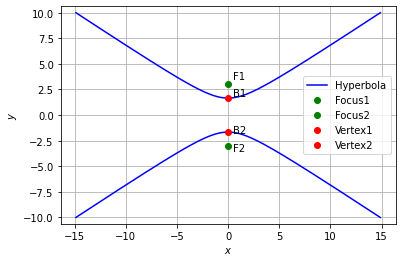
\includegraphics[width=\columnwidth]{hyperbola_plot.png}
\caption{Plot of Hyperbola}
\label{fig:hyperbola}
\end{figure}
\end{frame}
\end{document}